\chapter{Operations and Deployment}

\section{Packaging Strategy}
\begin{itemize}
    \item Ship as a single static binary where possible.
    \item Provide systemd service files and Windows service registration.
    \item Publish container images for controller-only deployments.
\end{itemize}

\section{Observability}
Tracing spans (via \texttt{tracing}) should cover API calls, AI requests, and adapter lifecycle. Emit metrics (latency, errors, probe results) to Prometheus or OpenTelemetry.

\section{Platform Notes}
\begin{itemize}
    \item \textbf{Windows}: install as a service using NSSM or native service wrapper; open firewall for control-plane port.
    \item \textbf{Linux}: ship systemd units with CapabilityBoundingSet for least privilege.
    \item \textbf{macOS}: use launchd plist; notarize binaries for distribution.
\end{itemize}

\section{Rollout Playbook}
\begin{enumerate}
    \item Stage in a non-critical region; collect probes.
    \item Gradually shift traffic using weighted rules.
    \item Roll back by restoring previous TOML snapshot.
\end{enumerate}

\section{Reference Deployment Diagram}
\begin{figure}[h]
    \centering
    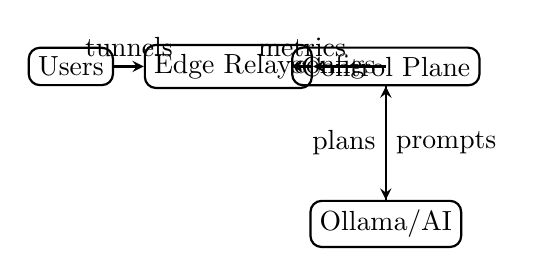
\begin{tikzpicture}[node distance=2cm,>=stealth,thick]
        \node (users) [draw, rounded corners] {Users};
        \node (edge) [draw, rounded corners, right of=users] {Edge Relays};
        \node (ctrl) [draw, rounded corners, right of=edge] {Control Plane};
        \node (ai) [draw, rounded corners, below of=ctrl] {Ollama/AI};
        \draw[->] (users) -- node[above]{tunnels} (edge);
        \draw[->] (edge) -- node[above]{metrics} (ctrl);
        \draw[->] (ctrl) -- node[right]{prompts} (ai);
        \draw[->] (ai) -- node[left]{plans} (ctrl);
        \draw[->] (ctrl) |- node[left]{configs} (edge);
    \end{tikzpicture}
    \caption{Operational layout with control plane driving edge relays.}
\end{figure}

